% Biên dịch từ thư mục baocao1 bằng XeLaTeX (hai lần).
% Ví dụ: xelatex bao_cao_tien_do.tex
% Toàn bộ ảnh được đóng gói trong baocao1/figures, không cần workspace gốc.
\documentclass[12pt,a4paper]{article}
\usepackage{fontspec}
\IfFontExistsTF{TeX Gyre Termes}{\setmainfont{TeX Gyre Termes}}{\setmainfont{DejaVu Serif}}
\IfFontExistsTF{TeX Gyre Heros}{\setsansfont{TeX Gyre Heros}}{\setsansfont{DejaVu Sans}}
\IfFontExistsTF{Latin Modern Mono}{\setmonofont{Latin Modern Mono}}{\setmonofont{DejaVu Sans Mono}}
\usepackage[vietnamese]{babel}
\usepackage[left=2.5cm,right=2.2cm,top=2.3cm,bottom=2.3cm]{geometry}
\usepackage{amsmath,amssymb,booktabs,tabularx,array,longtable}
\usepackage{graphicx,float,pdflscape,caption,enumitem,setspace,xcolor}
\usepackage[unicode,breaklinks,colorlinks=true,linkcolor=blue!45!black,citecolor=blue!45!black,urlcolor=blue!45!black]{hyperref}
\usepackage{xurl}
\graphicspath{{figures/}}
\setstretch{1.15}
\setlength{\parindent}{1.2em}
\setlength{\parskip}{0.25em}
\setlength{\emergencystretch}{3em}
\setlist{itemsep=0.2em,topsep=0.35em}
\captionsetup{font=small,labelfont=bf}
\renewcommand{\arraystretch}{1.18}
\newcolumntype{Y}{>{\raggedright\arraybackslash}X}
\newcommand{\FOUND}{\texttt{FOUND}}
\newcommand{\risk}{r_{\mathrm{err}}}
\newcommand{\srcpath}[1]{\begingroup\small\urlstyle{same}\path{#1}\endgroup}
\newcommand{\reportfigure}[4]{%
  \begin{figure}[H]\centering
    \includegraphics[width=#2\linewidth]{figures/#1}
    \caption{#3}\label{#4}
  \end{figure}}
\title{\textbf{BÁO CÁO Kết quả  ĐỒ ÁN}\\[0.7em]
\large Nghiên cứu phương pháp suy luận không gian và hiệu chuẩn độ bất định cho Spatial Vision--Language Model trong thao tác robot}
\author{Hệ thống nghiên cứu: P-CRA-U}
\date{Ngày 5 tháng 10 năm 2026}


\begin{document}
\maketitle
\begin{abstract}
Đồ án nghiên cứu hệ thống định vị thị giác--ngôn ngữ RGB-D có khả năng đánh giá bằng chứng không gian, ước lượng độ bất định và hiệu chuẩn xác suất lỗi để hỗ trợ quyết định chọn lọc cho robot. Kiến trúc P-CRA-U sử dụng backbone RoboRefer đóng băng, Sidecar dự đoán target và anchor, nhánh answerability, phép kiểm chứng quan hệ hình học và calibrator độc lập. Phương pháp ước lượng bất định sử dụng Monte Carlo Dropout (MC Dropout), tham khảo Gal và Ghahramani (ICML 2016), cùng mô hình likelihood cho nhiệm vụ thị giác theo Kendall và Gal (NeurIPS 2017).

Kết quả định vị đạt point-in-target 92,81\%, so với 86,71\% của RoboRefer. Tỉ lệ chấp nhận tăng từ 25,50\% lên 36,10\% khi điều chỉnh chính sách chọn lọc. Tại ngưỡng risk 0,2612, hệ thống nhận 36,10\% số mẫu với tỉ lệ lỗi 9,42\%; AURC đạt 0,2557. Các kết quả cho thấy lợi ích của việc kết hợp định vị với đánh giá khả năng trả lời và chọn lọc quyết định, đồng thời thể hiện đánh đổi giữa mức độ chấp nhận và rủi ro.
\end{abstract}
\tableofcontents
\clearpage

\section{Bài toán và mục tiêu nghiên cứu}
\subsection{Khoảng trống nghiên cứu}
Một hệ thống grounding xuất tọa độ chưa đủ thông tin để robot quyết định thực thi. Khi đối tượng không tồn tại, có nhiều đối tượng giống nhau, ảnh bị che khuất hoặc dữ liệu độ sâu thiếu tin cậy, một điểm dự đoán vẫn có thể được tạo ra. Nếu tầng lập kế hoạch sử dụng trực tiếp điểm đó, robot có thể chọn sai đối tượng.

Đồ án đặt vấn đề đánh giá đồng thời \emph{vị trí dự đoán}, \emph{khả năng trả lời từ quan sát hiện có} và \emph{mức rủi ro của việc chấp nhận dự đoán}. Hệ thống cần tận dụng thông tin RGB, depth và câu lệnh, đồng thời giữ khả năng từ chối hoặc yêu cầu thêm thông tin khi bằng chứng chưa đủ.

\subsection{Mục tiêu}
Mục tiêu trọng tâm là xây dựng và đánh giá hệ thống định vị thị giác--ngôn ngữ RGB-D có khả năng ước lượng độ bất định và hiệu chuẩn rủi ro phục vụ quyết định chọn lọc. Các công việc chính gồm:
\begin{enumerate}
\item Xây dựng Sidecar khai thác đặc trưng RGB/depth từ backbone đóng băng để định vị target và anchor.
\item Biểu diễn câu lệnh thành target, relation và anchor, rồi kiểm chứng ràng buộc không gian trên các đối tượng dự đoán.
\item Mô hình hóa các đại lượng bất định về ngữ nghĩa, vị trí, quan hệ, độ sâu và reference completion dưới che khuất.
\item Hiệu chuẩn bằng chứng thành xác suất lỗi nhận thức và lựa chọn giữa nhận dự đoán, quan sát lại, hỏi người dùng hoặc từ chối.
\end{enumerate}

\begin{landscape}
\begin{figure}[H]\centering
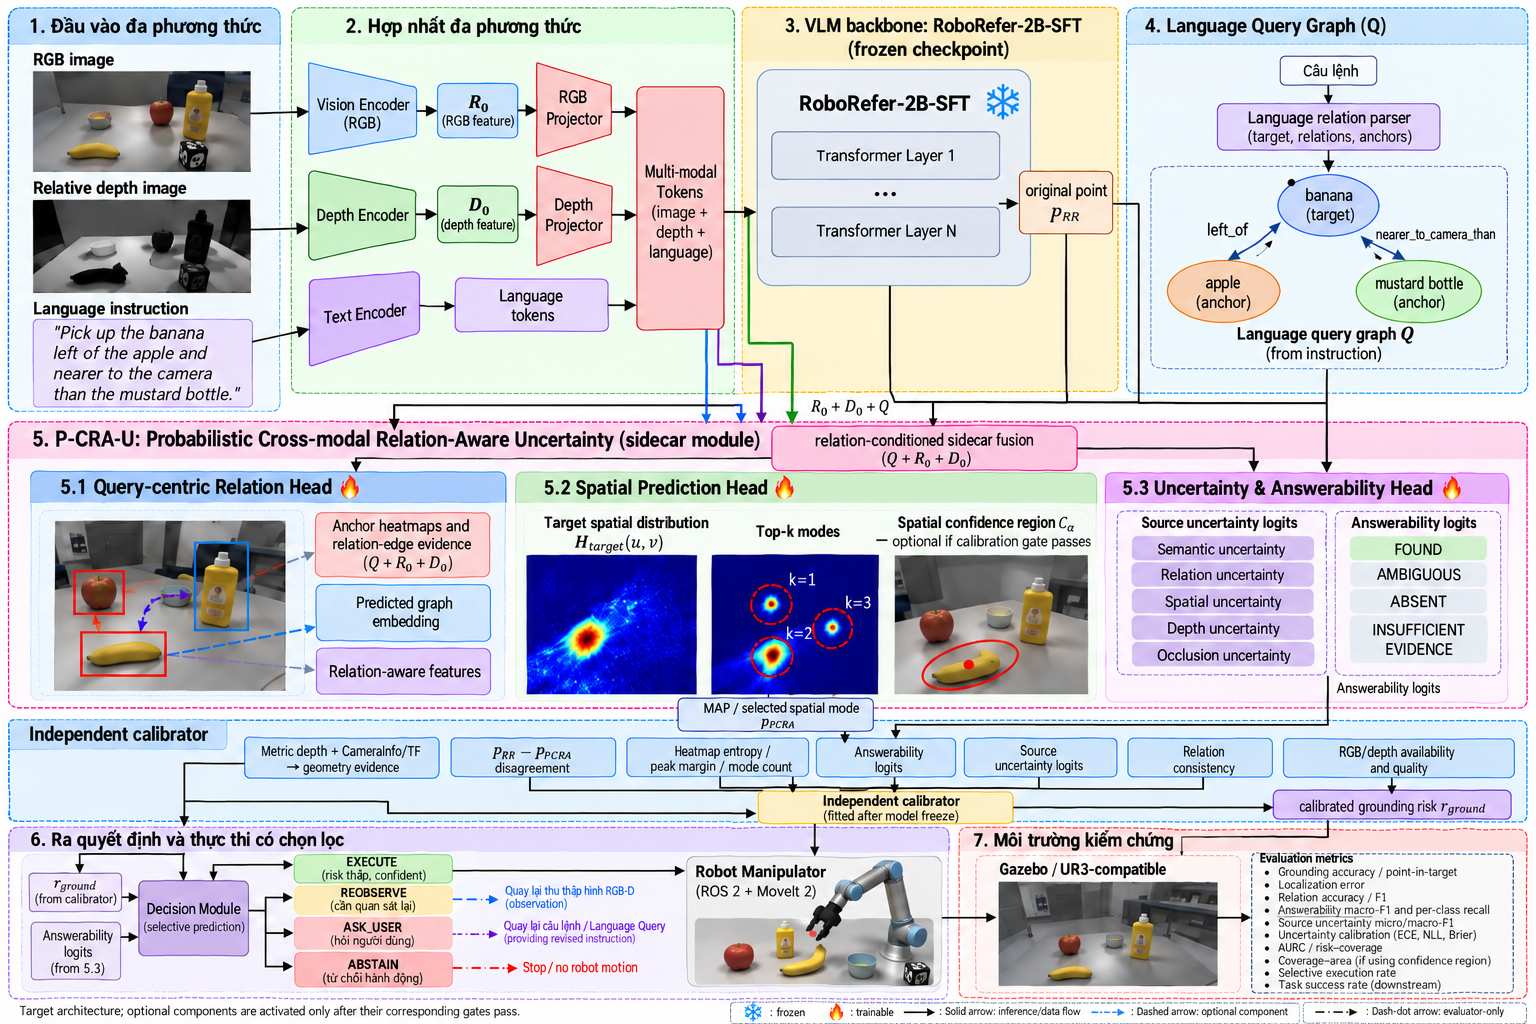
\includegraphics[width=0.98\linewidth,height=0.83\textheight,keepaspectratio]{figures/ppt_slide_04_image_01.png}
\caption{Sơ đồ kiến trúc tổng thể P-CRA-U.}
\label{fig:pipeline}
\end{figure}
\end{landscape}

\section{Phương pháp và công việc đã triển khai}
\subsection{Kiến trúc P-CRA-U}
Kiến trúc trong Hình~\ref{fig:pipeline} gồm đầu vào RGB-D và ngôn ngữ, backbone RoboRefer đóng băng, Sidecar phân tích đối tượng--quan hệ, các đầu ra không gian và answerability, calibrator độc lập và tầng quyết định chọn lọc. Nhánh suy luận hiện triển khai phép kiểm chứng trái/phải trong hệ tọa độ ảnh. Tầng quyết định xuất kết quả ở mức nhận thức để cung cấp cho hệ robot.

Luồng xử lý của phương pháp gồm:
\begin{center}\small
RGB-D + câu lệnh\\
$\downarrow$\\
Backbone đóng băng + Sidecar định vị\\
$\downarrow$\\
Target/anchor + parser + kiểm chứng quan hệ\\
$\downarrow$\\
Bằng chứng nhiệm vụ + uncertainty từ MC Dropout\\
$\downarrow$\\
Calibrator $\longrightarrow$ risk + quyết định.
\end{center}

\subsection{Đặc trưng đa phương thức và Sidecar}
Sidecar sử dụng RGB/depth features trước projector của RoboRefer, với kích thước mỗi grid $24\times32\times1152$. Backbone giữ đóng băng để tận dụng biểu diễn thị giác đã học. Text module riêng dùng token embeddings và Transformer để tạo biểu diễn câu lệnh có ngữ cảnh. Các slots target, relation và anchor cross-attend vào text tokens để hình thành queries phục vụ định vị.

RGB và depth đi qua các phép chiếu, sau đó hợp nhất bằng relation-conditioned gate và cross-modal residual blocks. Các spatial heads tạo target, interior và anchor heatmaps. Từ heatmaps, hệ thống trích MAP, các mode không gian và bằng chứng về sự tập trung của phân bố. Graph embedding và relation-edge head bổ sung biểu diễn đối tượng--quan hệ cho nhánh answerability.

Trong huấn luyện, heatmaps sử dụng BCE kết hợp Dice loss; answerability sử dụng cross-entropy; các nhánh evidence dùng các loss phù hợp với nhãn supervision. Ground-truth masks chỉ tham gia loss hoặc hậu kiểm, không được đưa vào inference.

\subsection{Nhánh answerability và Adapter}
Answerability phân loại đầu vào thành bốn trạng thái:
\begin{itemize}
\item \texttt{FOUND}: có thể định vị đối tượng từ bằng chứng quan sát.
\item \texttt{AMBIGUOUS}: có nhiều khả năng phù hợp, cần làm rõ yêu cầu.
\item \texttt{ABSENT}: đối tượng yêu cầu không có trong quan sát.
\item \texttt{INSUFFICIENT\_EVIDENCE}: bằng chứng hiện tại chưa đủ để trả lời.
\end{itemize}
Adapter \texttt{detail\_cost} sử dụng observable detail evidence để điều chỉnh answerability trong khi giữ phần định vị đóng băng. Cách tổ chức này cho phép nghiên cứu khả năng trả lời và quyết định chọn lọc mà không phải huấn luyện lại backbone.

\subsection{Parser target--relation--anchor}
Parser trích target phrase, anchor phrase, predicate và reference frame, đồng thời xác định vị trí token của các phrases. Với câu ``locate the apple that is right of the purple cube'', target là ``apple'', anchor là ``purple cube'' và quan hệ là \texttt{right\_of}. Phạm vi hiện hỗ trợ định vị trực tiếp và một quan hệ trái/phải trong ảnh. Câu ngoài phạm vi được đánh dấu unsupported.

Anchor query được điều kiện hóa theo cụm danh từ của đối tượng tham chiếu:
\begin{equation}
q_{\mathrm{new}}=q_{\mathrm{old}}+\mathrm{MLP}\!\left(\frac{1}{|A|}\sum_{j\in A}h_j\right),
\end{equation}
trong đó $A$ là tập token của anchor phrase và $h_j$ là contextual embedding. Residual MLP có 33.024 tham số, lớp cuối khởi tạo zero để bảo toàn đầu ra ban đầu. Nhánh mới sử dụng anchor head đóng băng để tạo anchor map.

Loss cho anchor kết hợp heatmap supervision với peak-aware constraints. Khi anchor nhìn thấy, margin loss khuyến khích peak trong mask cao hơn peak ngoài mask. Khi anchor không có support quan sát, penalty trên max logit bổ sung cho zero-map BCE nhằm hạn chế peak giả. Masks chỉ dùng trong huấn luyện và đánh giá.

\subsection{Kiểm chứng hình học quan hệ}
Phương pháp tham khảo cách tách hình thức hóa yêu cầu khỏi tính toán hình học trong GCA~\cite{gca}. Sau khi xác định target và anchor, verifier kiểm tra ràng buộc trên vị trí dự đoán.

Với target peak $(t_x,t_y)$ và anchor peak $(a_x,a_y)$, đặt $s=+1$ cho \texttt{right\_of}, $s=-1$ cho \texttt{left\_of}. Signed margin là
\begin{equation}
m=s(t_x-a_x)-12\ \mathrm{px}.
\end{equation}
Hai peaks tương thích khi $m>0$. Với các maps chuẩn hóa $P_T,P_A$, mức tương thích phân bố là
\begin{equation}\label{eq:relation}
c=\sum_i\sum_jP_T(i)P_A(j)\,\mathbf1\{s(x_i-x_j)>12\}.
\end{equation}
Công thức dùng xấp xỉ tích hai marginal maps. Margin và compatibility được đưa vào bằng chứng cho calibrator. Hệ thống giữ riêng evidence về sự hiện diện và danh tính của anchor, vì kiểm tra quan hệ hình học còn phụ thuộc việc chọn đúng đối tượng. Verifier cung cấp evidence, không trực tiếp thay target MAP.

\subsection{Cơ sở ước lượng bất định}
\textbf{Phương pháp tham khảo Kendall \& Gal, NeurIPS 2017}~\cite{kendall2017}, về mô hình uncertainty cho semantic segmentation và depth regression. \textbf{MC Dropout dựa trên Gal \& Ghahramani, ICML 2016}~\cite{gal2016}; đại lượng mutual information tham khảo Gal, Islam \& Ghahramani, ICML 2017~\cite{gal2017}.

Aleatoric uncertainty liên quan biến thiên có điều kiện trong quan sát/đầu ra; epistemic uncertainty liên quan sự thiếu chắc chắn của mô hình. Trong phương pháp, likelihood mô hình hóa phân bố đầu ra, còn MC Dropout tạo nhiều dự đoán để đo disagreement. Backbone và query representations giữ cố định; việc lấy mẫu tập trung vào fusion và task heads có dropout.

Hệ thống thực hiện $T=20$ stochastic forward passes với dropout $p=0{,}1$. Với đầu ra categorical $p_t(k)$ của lần lấy mẫu $t$, tính
\begin{align}
\bar p(k)&=\frac1T\sum_{t=1}^{T}p_t(k),\\
H(p)&=-\frac{\sum_{k=1}^{K}p(k)\log p(k)}{\log K},\\
U_{\mathrm{PE}}&=H(\bar p),\\
U_{\mathrm{EE}}&=\frac1T\sum_tH(p_t),\\
U_{\mathrm{MI}}&=H(\bar p)-\frac1T\sum_tH(p_t).
\end{align}
PE là entropy của predictive mixture; EE là entropy trung bình của các dự đoán; MI phản ánh disagreement giữa các lần lấy mẫu mô hình. Với biến Bernoulli, dùng $K=2$ và vector $(1-c_t,c_t)$. Các đại lượng được hiểu trong phạm vi các nhánh đã lấy mẫu.

\subsection{Cách đo bất định theo năm nhóm nhiệm vụ}
\subsubsection{Ngữ nghĩa: semantic identity}
Semantic head nhận RGB projection 128 chiều, dùng LayerNorm, MLP, GELU và Dropout để dự đoán phân bố 22 lớp, gồm background và 21 lớp đối tượng. Head được học bằng categorical cross-entropy từ semantic-instance annotations.

Tại vị trí target/anchor dự đoán, phân bố lớp được lấy qua các MC draws để tính entropy và MI. Noun score là xác suất lớp tương ứng cụm danh từ khi phrase thuộc catalog. Đại lượng này đo bất định nhận dạng lớp tại node được chọn; phân biệt các instances cùng lớp vẫn cần thêm bằng chứng binding.

\subsubsection{Không gian: spatial localization}
Mỗi MC draw tạo fused visual representation khác nhau, từ đó tạo target và anchor maps qua các heads đóng băng. Spatial softmax chuẩn hóa logits trên 768 grid cells. Entropy mô tả độ phân tán vị trí; MI mô tả disagreement giữa maps. Các maps được sử dụng như biểu diễn bất định vị trí, cùng với peak và các bằng chứng quan sát khác.

\subsubsection{Quan hệ: relation compatibility}
Tính compatibility $c_t$ theo Công thức~\eqref{eq:relation} cho từng MC draw. Phân bố $(1-c_t,c_t)$ mô tả hai trạng thái không tương thích/tương thích của cặp vị trí dự đoán. PE và MI đo sự không chắc chắn của phép kiểm chứng trái/phải. Với câu direct hoặc unsupported, hệ thống không tạo một quan hệ giả để tính uncertainty.

\subsubsection{Độ sâu: depth regression}
Depth head nhận RGB/depth projections 256 chiều và dự đoán mean $\mu_t$, variance $\sigma_t^2>0$. Theo likelihood Gaussian được sử dụng trong hướng Kendall \& Gal, loss là
\begin{equation}
\mathcal L_{\mathrm{depth}}=\frac12\left[\frac{(z-\mu)^2}{\sigma^2}+\log\sigma^2+\log(2\pi)\right].
\end{equation}
Metric depth dùng làm supervision; inference dùng đặc trưng từ RGB và relative depth. Predictive distribution tại pixel dự đoán được xấp xỉ bằng Gaussian mixture:
\begin{equation}
p(z\mid x)\approx\frac1T\sum_t\mathcal N(z;\mu_t,\sigma_t^2).
\end{equation}
Tổng phương sai gồm hai thành phần:
\begin{equation}
\mathrm{Var}(z\mid x)=\underbrace{\frac1T\sum_t\sigma_t^2}_{\text{conditional variance}}+
\underbrace{\frac1T\sum_t(\mu_t-\bar\mu)^2}_{\text{MC mean variance}}.
\end{equation}
Khoảng dự đoán lấy từ quantiles của mixture. Conditional variance và MC mean variance được báo riêng để phân biệt độ phân tán của likelihood với disagreement của mô hình.

\subsubsection{Che khuất: reference completion}
Nhánh completion mô hình hóa phân bố vị trí trên reference support của target. Head nhận fused features, target phrase representation, target logit và tọa độ grid, rồi dự đoán residual logits. Loss là categorical cross-entropy với mask-area distribution:
\begin{equation}
q_i=\frac{a_i}{\sum_j a_j},\qquad
\mathcal L_{\mathrm{completion}}=-\sum_iq_i\log P_C(i).
\end{equation}
Trong đó $a_i$ là diện tích reference support trong cell. MC draws cho nhiều completion distributions để tính PE và MI; unobserved mass được tính từ predicted visible target map. Đây là mô hình reference completion dưới che khuất, không phải tái dựng đầy đủ hình dạng amodal.

\begin{table}[H]\centering\small
\caption{Các biến nhiệm vụ và đại lượng uncertainty của phương pháp.}
\begin{tabularx}{\linewidth}{p{2.2cm}Y Y}\toprule
Nhóm & Biến dự đoán & Đại lượng tính toán\\
\midrule
Semantic & Lớp đối tượng tại target/anchor node & Entropy, MC MI, noun score\\
Spatial & Vị trí target và anchor & Map entropy, MC disagreement\\
Relation & Tương thích quan hệ trái/phải & Bernoulli entropy, MC MI\\
Depth & Độ sâu tại pixel dự đoán & Conditional variance, MC variance, interval\\
Occlusion & Vị trí theo reference completion & Completion entropy, MC MI, unobserved mass\\
\bottomrule\end{tabularx}
\end{table}
Năm nhóm mô tả các biến nhiệm vụ khác nhau và có thể phụ thuộc nhau. Phương pháp không cộng chúng thành năm nguyên nhân độc lập. Bằng chứng uncertainty được kết hợp thông qua calibrator của xác suất lỗi.

\subsection{Hiệu chuẩn risk và quyết định chọn lọc}
Event lỗi nhận thức được định nghĩa:
\begin{equation}
e=\mathbf1\{y_{\mathrm{true}}\ne\FOUND\ \text{hoặc MAP ngoài target mask}\}.
\end{equation}
Calibrator nhận observable evidence như heatmap concentration, answerability, anchor evidence, relation compatibility, thông tin RGB-D và task uncertainty. Logistic calibration có dạng
\begin{equation}
\risk=\operatorname{sigmoid}\left(b+\sum_kw_k\frac{x_k-\mu_k}{s_k}\right).
\end{equation}
Model được freeze trước fit calibration; checkpoint chọn bằng dev, còn ngưỡng nhận chọn trên calibration. Ground-truth chỉ dùng để tạo event supervision và đánh giá. Việc đánh giá calibration tham khảo khái niệm confidence calibration của Guo et al.~\cite{guo2017}.

Policy Hard-FOUND nhận dự đoán khi predicted \FOUND\ và $\risk\le\tau$. Các trạng thái còn lại dẫn tới \texttt{ASK\_USER}, \texttt{REOBSERVE} hoặc \texttt{ABSTAIN}. Risk là xác suất lỗi nhận thức, không phải bốn khoảng để chia bốn actions. Tầng quyết định tạo tín hiệu chấp nhận/từ chối cho hệ robot.

\section{Kết quả thực nghiệm và đánh giá}
\subsection{Chất lượng grounding theo quan hệ}
\reportfigure{ppt_slide_05_image_02.png}{1.0}{So sánh point-in-target của RoboRefer và P-CRA-U theo nhóm quan hệ.}{fig:relations}
\begin{table}[H]\centering\small
\caption{Tỉ lệ định vị đúng theo quan hệ.}
\begin{tabular}{lrrr}\toprule
Quan hệ & Số mẫu & RoboRefer (\%) & P-CRA-U (\%)\\
\midrule
Direct &338&92,0&90,8\\
Left of &53&96,2&88,7\\
Right of &57&75,4&94,7\\
Front of &137&83,9&94,9\\
Behind &78&89,7&98,7\\
Nearer than &57&78,9&96,5\\
Farther than &46&76,1&95,7\\
Between in depth &30&90,0&76,7\\
Nearer than both &39&69,2&97,4\\
\bottomrule\end{tabular}
\end{table}
P-CRA-U cải thiện ở phần lớn các nhóm quan hệ. Mức tăng nổi bật xuất hiện ở right-of, farther-than và nearer-than-both. Các nhóm front-of, behind và nearer-than cũng cho tỉ lệ định vị đúng cao hơn RoboRefer. Điều này cho thấy hệ thống khai thác được thông tin đối tượng và quan hệ để hỗ trợ grounding.

Kết quả chưa đồng đều: direct, left-of và between-in-depth thấp hơn đối chứng. Between-in-depth giảm từ 90,0\% xuống 76,7\%, là nhóm cần ưu tiên phân tích thêm. Các nhóm có ít mẫu cũng cần được đánh giá thận trọng. Biểu đồ phản ánh khả năng định vị trên câu lệnh có quan hệ, không trực tiếp đo độ chính xác của từng đại lượng uncertainty.

\subsection{Chất lượng grounding theo biến thể dữ liệu}
\reportfigure{ppt_slide_06_image_03.png}{0.96}{Point-in-target theo điều kiện đầu vào và các biến thể counterfactual.}{fig:variants}
\begin{table}[H]\centering\small
\caption{Tỉ lệ định vị đúng theo biến thể dữ liệu.}
\begin{tabular}{lrrr}\toprule
Biến thể & Số mẫu & RoboRefer (\%) & P-CRA-U (\%)\\
\midrule
Clean &154&83,1&90,9\\
Semantic counterfactual &200&96,0&99,5\\
Relation counterfactual &173&89,6&94,8\\
Depth corruption &154&81,2&88,3\\
Occlusion/view counterfactual &154&80,5&88,3\\
\bottomrule\end{tabular}
\end{table}
P-CRA-U có tỉ lệ định vị đúng cao hơn trên cả năm biến thể. Với dữ liệu clean, mức tăng là 7,8 điểm phần trăm. Khi depth bị suy giảm chất lượng hoặc góc nhìn/che khuất thay đổi, P-CRA-U vẫn đạt 88,3\%, cao hơn đối chứng lần lượt khoảng 7,1 và 7,8 điểm phần trăm. Kết quả cho thấy chất lượng grounding được duy trì tốt hơn trong các điều kiện quan sát khó của bộ dữ liệu.

Semantic counterfactual đạt 99,5\% và relation counterfactual đạt 94,8\%. Tuy nhiên, point-in-target chỉ kiểm tra vị trí nằm trong target mask; việc chấp nhận dự đoán còn phụ thuộc answerability và risk. Vì vậy cần xem các kết quả này cùng với đánh giá chọn lọc ở các mục tiếp theo.

\subsection{So sánh tổng thể với phương pháp đối chứng}
\reportfigure{ppt_slide_07_image_04.png}{1.0}{So sánh tổng thể RoboRefer RGB-D, P-CRA-U V2 và P-CRA-U có Adapter.}{fig:comparison}
Point-in-target của P-CRA-U đạt 92,81\%, so với 86,71\% của RoboRefer, tương ứng mức tăng khoảng 6,10 điểm phần trăm theo các giá trị làm tròn trong bảng. Việc bổ sung Adapter tập trung vào answerability và quyết định chọn lọc trong khi giữ chất lượng định vị.

False-FOUND giảm từ 0,1207 xuống 0,0948 giữa P-CRA-U V2 và P-CRA-U có Adapter. Điều này cho thấy hệ thống giảm việc kết luận có thể trả lời ở các ca thực tế không đủ điều kiện. Đồng thời, coverage tăng từ 0,2550 lên 0,3610, tức nhận thêm dự đoán thay vì chỉ tăng từ chối.

Coverage 1,0000 của RoboRefer thể hiện cách xuất kết quả không có cơ chế selective rejection tương ứng. Do đó, coverage cần đọc cùng chất lượng định vị và tỉ lệ lỗi, không xem mức nhận cao nhất luôn là lựa chọn tốt nhất.

\subsection{Ảnh hưởng của chính sách chọn lọc}
Chính sách ban đầu đặt budget lỗi trên calibration là 5,0\%, với ngưỡng risk khoảng 0,0937. Hệ thống nhận 255/1.000 mẫu, coverage 25,50\% và valid recall 61,48\%. Cách chọn này ưu tiên thận trọng nhưng từ chối nhiều ca hợp lệ.

Khi chuyển sang Hard-FOUND và budget calibration 7,5\%, ngưỡng risk là 0,2612. Coverage tăng lên 36,10\%, valid recall đạt 80,74\% và giữ lại thêm 78 ca định vị đúng. Các số cho thấy khả năng thu hồi ca hợp lệ tốt hơn khi điều chỉnh chính sách.

\begin{table}[H]\centering
\caption{Đánh đổi mức chấp nhận trước và sau điều chỉnh chính sách.}
\begin{tabular}{lrr}\toprule
Chỉ số & Trước điều chỉnh & Sau điều chỉnh\\
\midrule
Budget trên calibration &5,0\%&7,5\%\\
Ngưỡng risk &0,0937&0,2612\\
Số mẫu nhận / 1.000 &255&361\\
Coverage &25,50\%&36,10\%\\
Valid recall &61,48\%&80,74\%\\
\bottomrule\end{tabular}
\end{table}
Budget 7,5\% là mục tiêu chọn ngưỡng trên calibration. Tỉ lệ lỗi thực nghiệm tại điểm vận hành là 9,42\%, cho thấy vẫn còn khoảng cách giữa mục tiêu và kết quả đánh giá. Việc tăng khả năng chấp nhận cần được xem là đánh đổi với rủi ro, thay vì chỉ đánh giá qua coverage.

\subsection{Đường risk--coverage và AURC}
\reportfigure{ppt_slide_09_image_05.png}{0.94}{Đường risk--coverage và điểm vận hành của chính sách chọn lọc.}{fig:riskcoverage}
Trục ngang biểu diễn tỉ lệ mẫu được chấp nhận; trục dọc là tỉ lệ lỗi trong tập nhận. Khi sắp dự đoán theo risk tăng dần, hệ thống ưu tiên các ca có evidence đáng tin hơn. Đường cong cho thấy risk nhìn chung tăng khi mở rộng tập nhận, thể hiện đánh đổi giữa coverage và chất lượng dự đoán.

Tại ngưỡng 0,2612, policy nhận 36,1\% mẫu với risk thực nghiệm 9,42\%. Đường tham chiếu toàn bộ mẫu có tỉ lệ lỗi 59,5\%; sự khác biệt cho thấy chọn lọc giúp tập được nhận có tỉ lệ lỗi thấp hơn việc nhận toàn bộ. Điểm vận hành còn yêu cầu predicted FOUND, kết hợp khả năng trả lời với risk.

AURC đạt 0,2557, tổng hợp chất lượng xếp hạng theo toàn bộ mức coverage. Chỉ số này cần được hiểu trên cùng dataset và định nghĩa lỗi. Kết quả thể hiện khả năng ưu tiên các dự đoán ít lỗi hơn, đồng thời cho thấy risk vẫn tăng khi cần nhận nhiều mẫu hơn.

\section{Kết luận tiến độ và hướng tiếp tục}
\subsection{Kết luận}
Đồ án đã xây dựng kiến trúc P-CRA-U kết hợp backbone RGB-D đóng băng, Sidecar định vị và answerability, biểu diễn target--relation--anchor, kiểm chứng quan hệ hình học, ước lượng uncertainty nhiệm vụ bằng MC Dropout và hiệu chuẩn xác suất lỗi. Kendall \& Gal (NeurIPS 2017) là cơ sở cho mô hình likelihood thị giác, còn Gal \& Ghahramani (ICML 2016) cung cấp nền tảng MC Dropout.

Các kết quả grounding cho thấy P-CRA-U đạt point-in-target 92,81\%, cao hơn RoboRefer 86,71\%, và cải thiện trên cả năm biến thể dữ liệu được đánh giá. Tuy nhiên, mức cải thiện theo quan hệ chưa đồng đều, đặc biệt ở left-of và between-in-depth.

Về quyết định chọn lọc, coverage tăng từ 25,50\% lên 36,10\%, valid recall tăng từ 61,48\% lên 80,74\%. Tại điểm vận hành, selective risk là 9,42\% và AURC là 0,2557. Kết quả cho thấy hệ thống có thể thu hồi nhiều ca hợp lệ hơn, nhưng vẫn cần giảm lỗi trong tập nhận để đáp ứng tốt hơn budget calibration.



\clearpage
\begin{thebibliography}{9}
\bibitem{kendall2017}
A. Kendall and Y. Gal, ``What Uncertainties Do We Need in Bayesian Deep Learning for Computer Vision?'', \emph{NeurIPS}, 2017.
\url{https://proceedings.neurips.cc/paper_files/paper/2017/file/2650d6089a6d640c5e85b2b88265dc2b-Paper.pdf}.
\bibitem{gal2016}
Y. Gal and Z. Ghahramani, ``Dropout as a Bayesian Approximation: Representing Model Uncertainty in Deep Learning'', \emph{ICML}, PMLR 48, pp. 1050--1059, 2016.
\url{https://proceedings.mlr.press/v48/gal16.html}.
\bibitem{gal2017}
Y. Gal, R. Islam and Z. Ghahramani, ``Deep Bayesian Active Learning with Image Data'', \emph{ICML}, PMLR 70, pp. 1183--1192, 2017.
\url{https://proceedings.mlr.press/v70/gal17a.html}.
\bibitem{gca}
Z. Chen et al., ``Geometrically-Constrained Agent for Spatial Reasoning'', \emph{CVPR}, 2026; arXiv:2511.22659, bản đầu năm 2025.
\url{https://arxiv.org/abs/2511.22659}.
\bibitem{guo2017}
C. Guo, G. Pleiss, Y. Sun and K. Q. Weinberger, ``On Calibration of Modern Neural Networks'', \emph{ICML}, PMLR 70, pp. 1321--1330, 2017.
\url{https://proceedings.mlr.press/v70/guo17a.html}.
\end{thebibliography}

\appendix




\end{document}
